
\documentclass[10pt,a4paper]{article}
\usepackage{times}
\usepackage{bm,bbm}
\usepackage{amsmath,amssymb,amsthm}
\usepackage{graphicx,subfigure}
\usepackage{url}
\usepackage{units}
\usepackage{cite,balance}
\usepackage{comment}
\usepackage{multirow}
\usepackage{booktabs}
\usepackage{microtype}
%\usepackage{siunitx}
\usepackage{color}
\usepackage{enumerate}
\usepackage{stackrel}
\usepackage{float}


\usepackage{geometry}
\geometry{
	a4paper,
	total={170mm,257mm},
	left=1cm,right=1cm,
	top=1cm,bottom=1.5cm
}



\usepackage[normalem]{ulem} %%%% para tachar texto


%%%%% THEOREMS %%%%%%%%%%%%%%%%%%%%%%%%%%%%%%%%%%%%%

\newtheorem{corollary}{Corollary}[section]
\newtheorem{lemma}{Lema}[section]
\newtheorem{theorem}{Theorem}[section]
\newtheorem{definition}{Definition}
\newtheorem{proposition}{Proposition}



\title{Filtros aplicados a una imagen sintética\\ Figure 5 (a) Chan et al. (2022)}
\date{}


\begin{document}

\maketitle


% Table generated by Excel2LaTeX from sheet 'Hoja1'
\begin{table}[htbp]
	\centering
	\caption{Add caption}
	\begin{tabular}{lrr}
		& \multicolumn{1}{c}{$\widehat{ENL}$} & \multicolumn{1}{c}{$\hat{\mu}$ } \\
		\midrule
		Noisy  & 0.574 & 6.212 \\
		Lee (3x3) & 2.665 & 6.210 \\
		Lee (5x5) & 3.845 & 6.211 \\
		Lee (7x7) & 4.829 & 6.211 \\
		Enhanced Lee & 4.497 & 5.571 \\
		FANS  & 0.003 & 15.676 \\
		Shannon Entropy  & 12.282 & 6.184 \\
		N1-h2-9x3 & 45.679 & 6.197 \\
		N1-h3-9x3 & 44.990 & 5.750 \\
		N1-h4-9x3 & 22.633 & 5.659 \\
		N1-h2-9x5 & 45.649 & 6.206 \\
		N1-h3-9x5 & 44.182 & 6.099 \\
		N1-h4-9x5 & 32.065 & 5.909 \\
		N1-h2-11x7 & 67.817 & 6.206 \\
		N1-h3-11x7 & 65.954 & 6.159 \\
		N1-h4-11x7 & 52.104 & 6.026 \\
	\end{tabular}%
	\label{tab:addlabel}%
\end{table}%



\newpage

\section{LEE}
\begin{figure}[H]
	\centering
	\subfigure[\label{CuatroZonas_Lee_3x3}$3x3$]{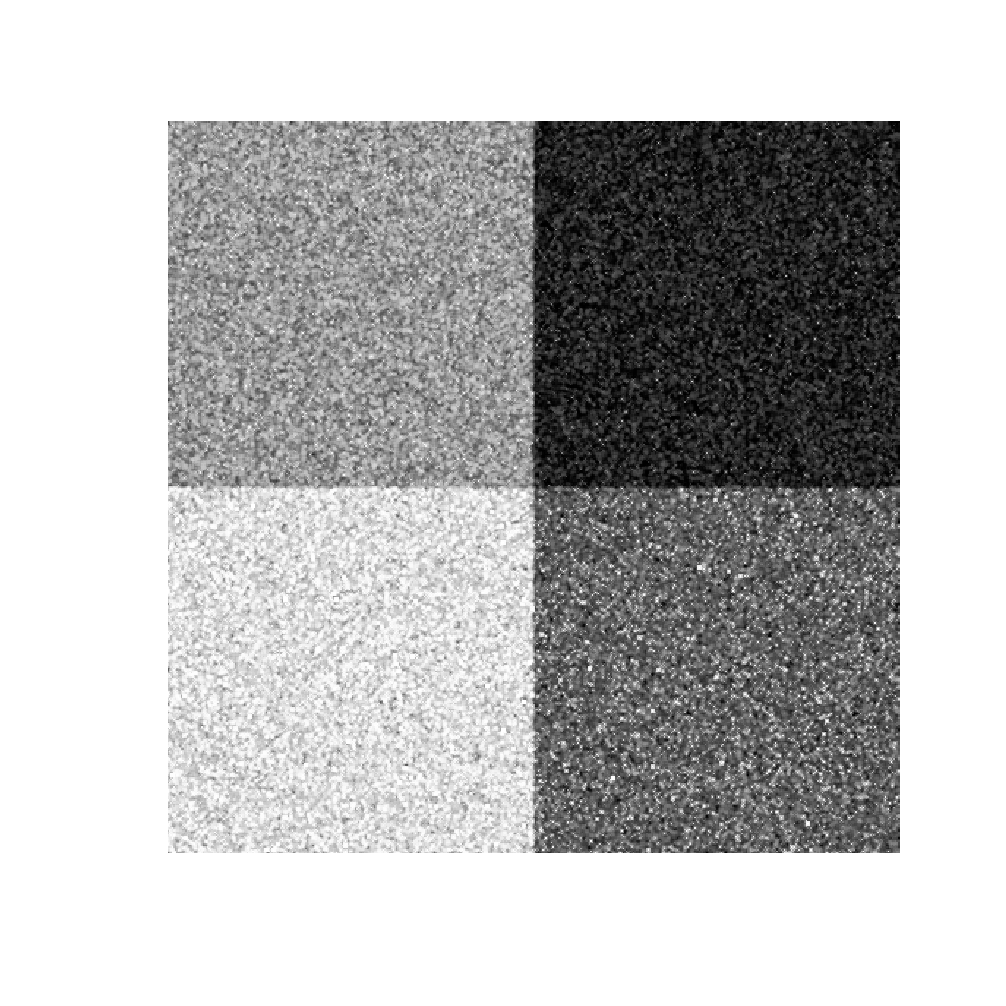
\includegraphics[scale=0.3]{../Figures/LEE/CuatroZonas_Lee_3x3.pdf}}
	\subfigure[\label{CuatroZonas_Lee_5x5}$5x5$]{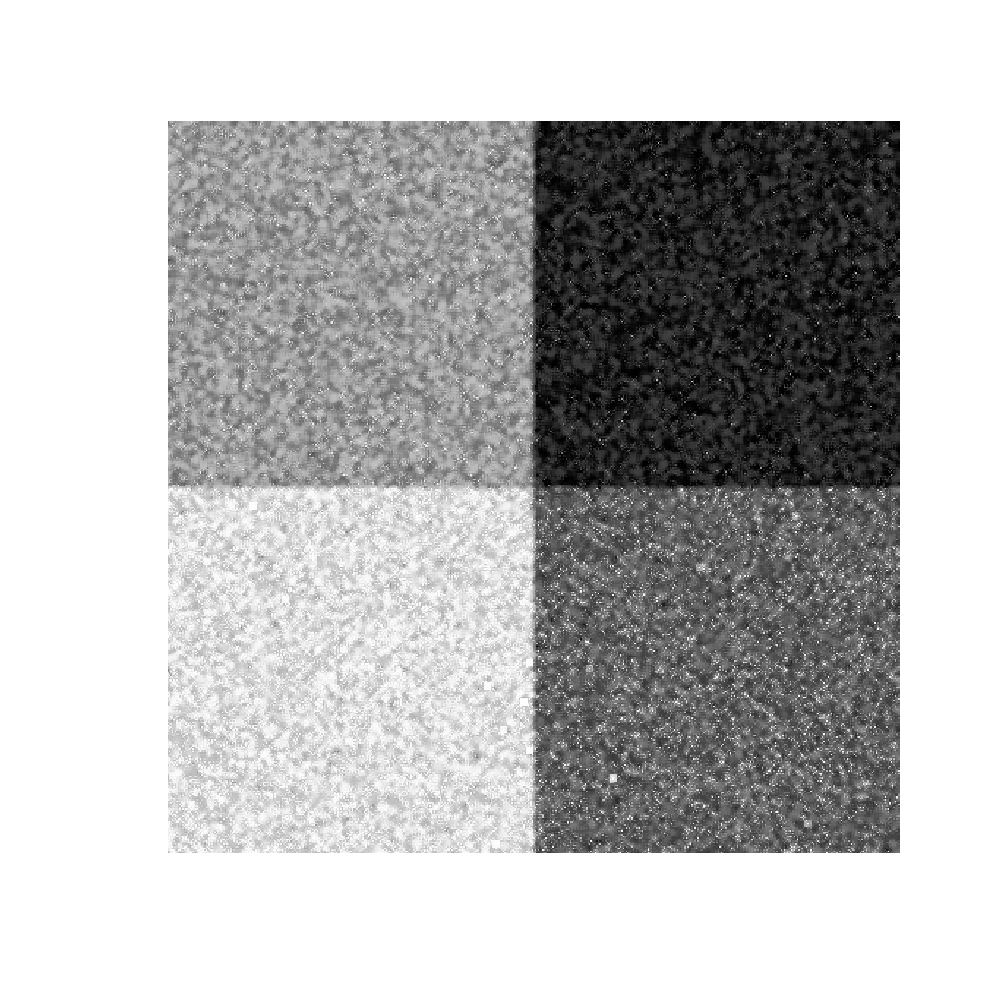
\includegraphics[scale=0.3]{../Figures/LEE/CuatroZonas_Lee_5x5.pdf}}
	\subfigure[\label{CuatroZonas_Lee_7x7}$7x7$]{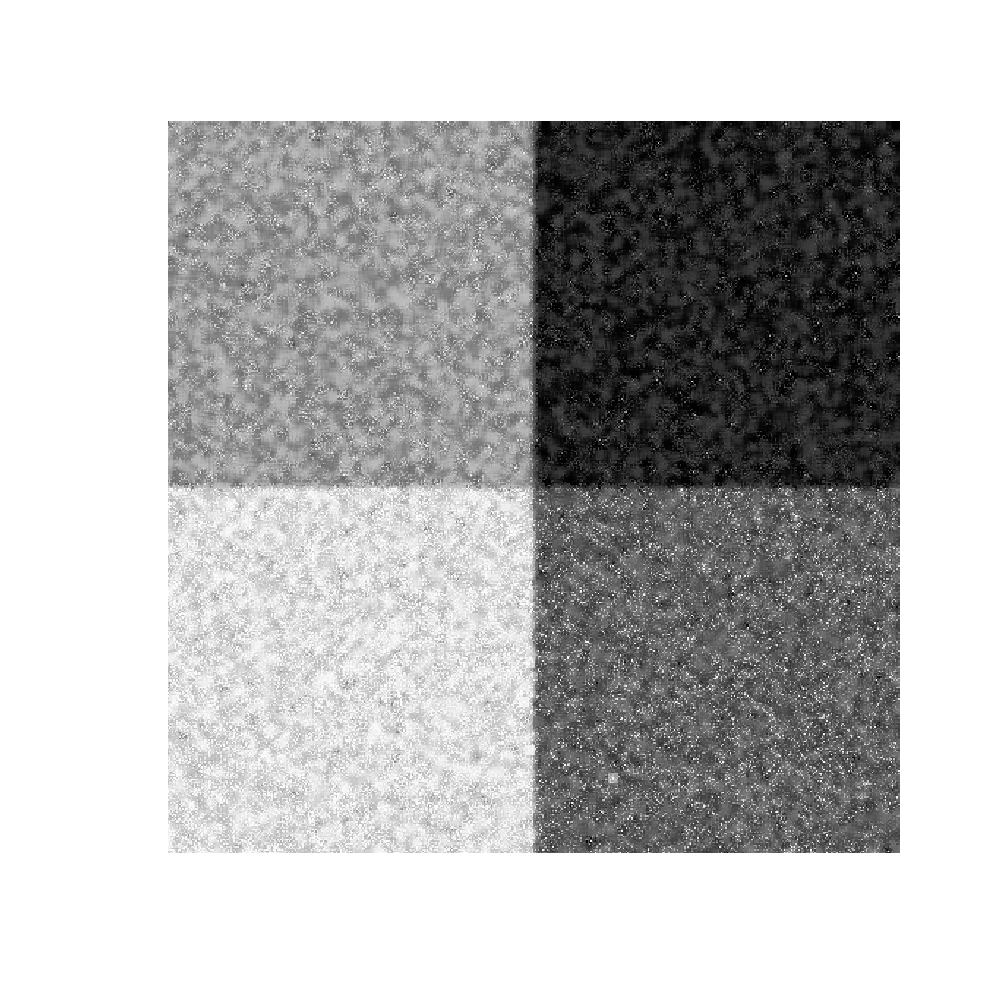
\includegraphics[scale=0.3]{../Figures/LEE/CuatroZonas_Lee_7x7.pdf}}
	\subfigure[\label{Cociente_CuatroZonas_Lee_3x3}Cociente $3x3$]{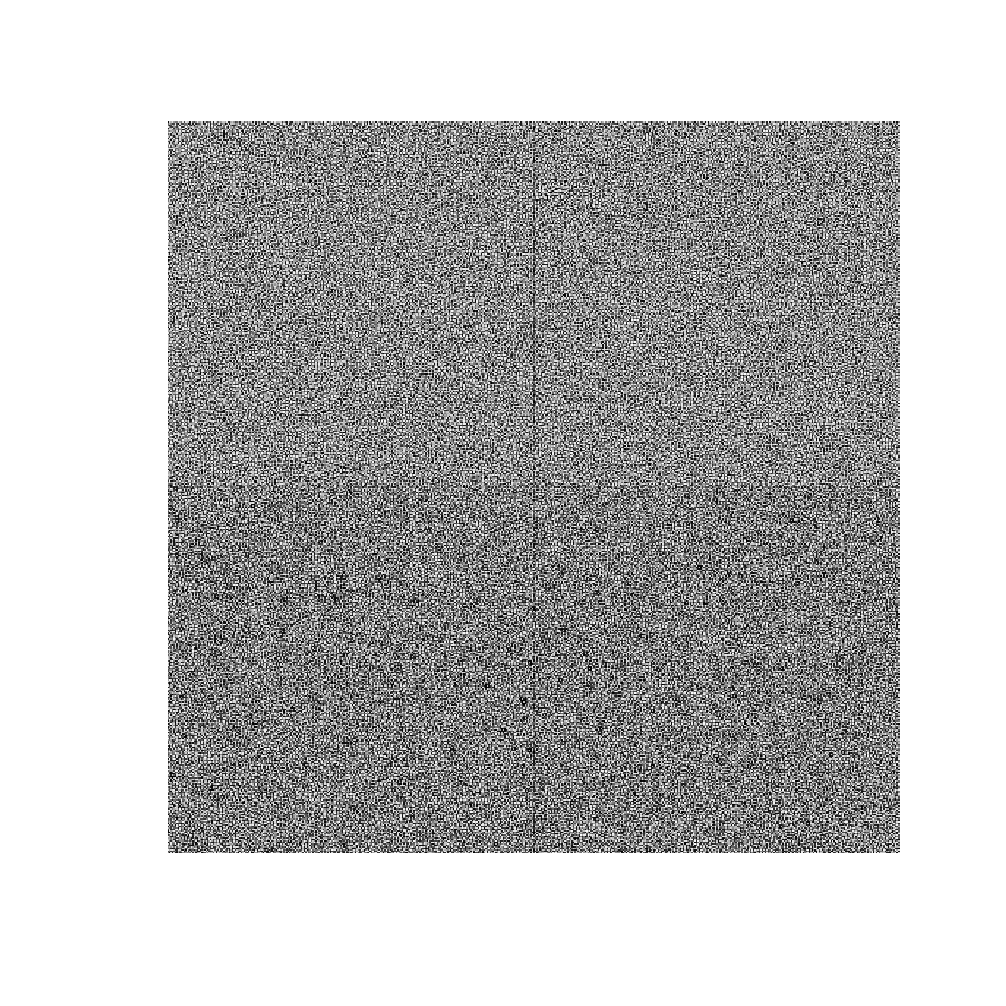
\includegraphics[scale=0.3]{../Figures/LEE/Cociente_CuatroZonas_Lee_3x3.pdf}}
	\subfigure[\label{Cociente_CuatroZonas_Lee_5x5}Cociente $5x5$]{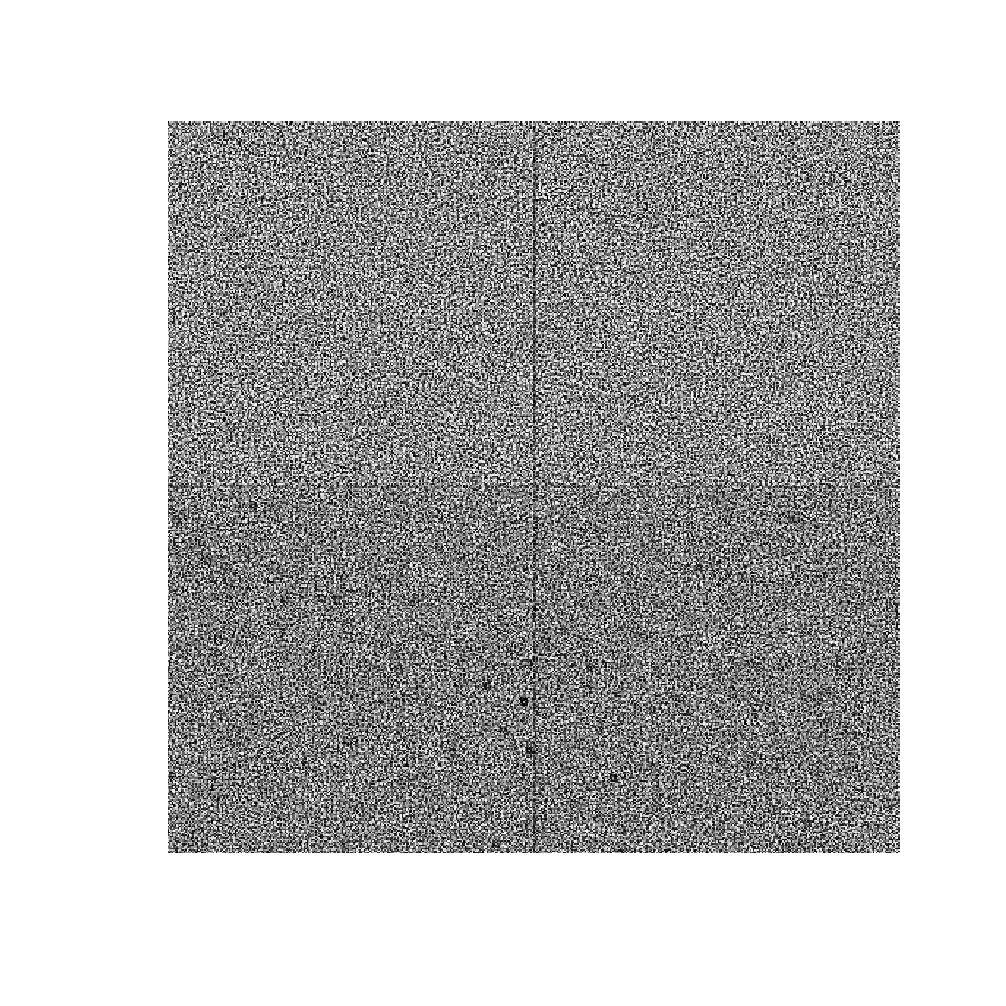
\includegraphics[scale=0.3]{../Figures/LEE/Cociente_CuatroZonas_Lee_5x5.pdf}}
	\subfigure[\label{Cociente_CuatroZonas_Lee_7x7}Cociente $7x7$]{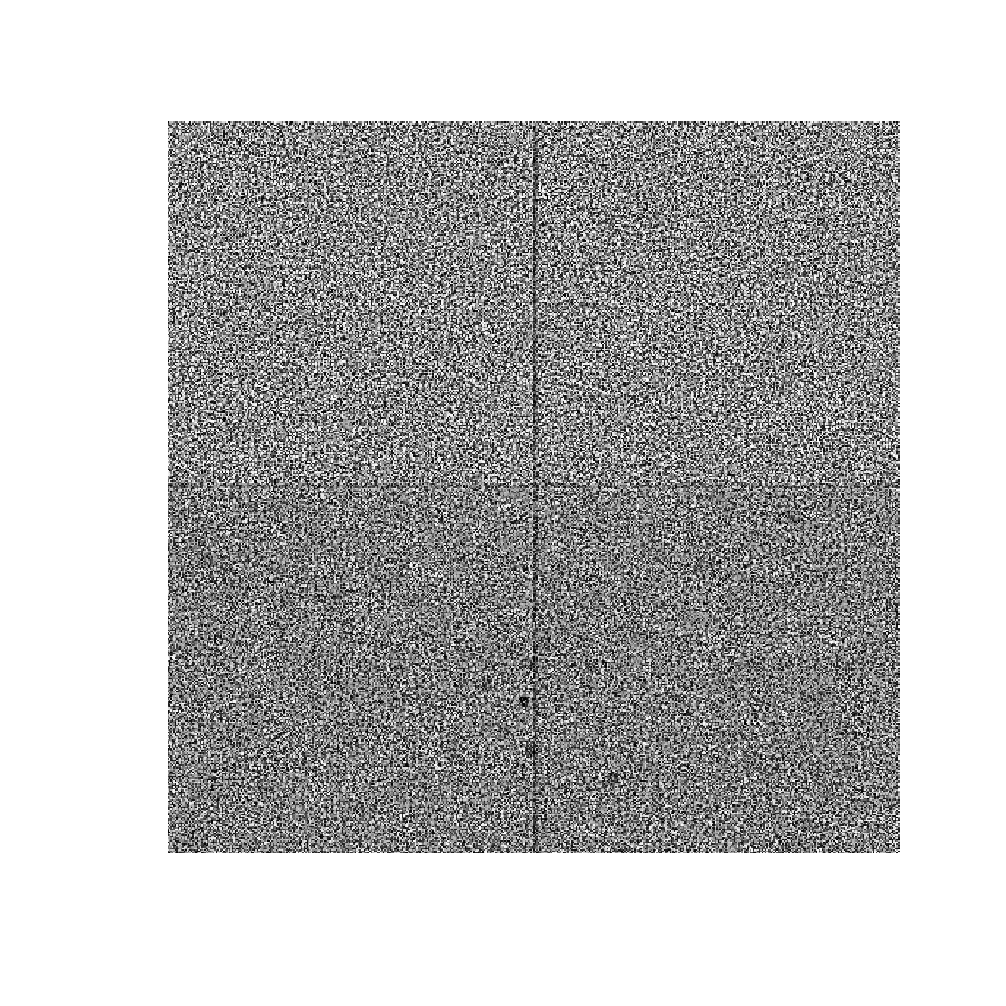
\includegraphics[scale=0.3]{../Figures/LEE/Cociente_CuatroZonas_Lee_7x7.pdf}}
	\caption{LEE}
\end{figure}  

\vspace{1cm}

\section{ENHANCED LEE}
\begin{figure}[H]
	\centering
	\subfigure[\label{CuatroZonas_EnhancedLee}$ Enhanced Lee$]{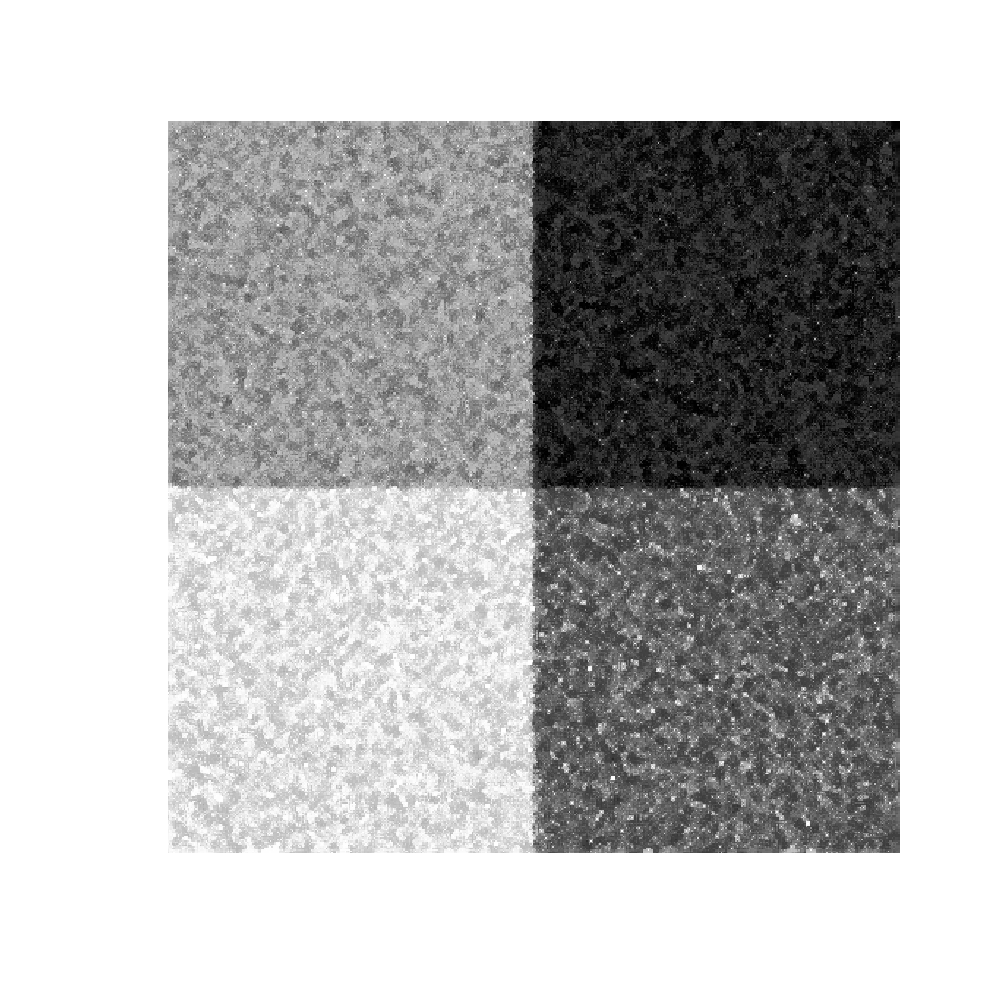
\includegraphics[scale=0.3]{../Figures/LEE/CuatroZonas_EnhancedLee.pdf}}
	\subfigure[\label{Cociente_CuatroZonas_EnhancedLee}Cociente $Enhanced Lee$]{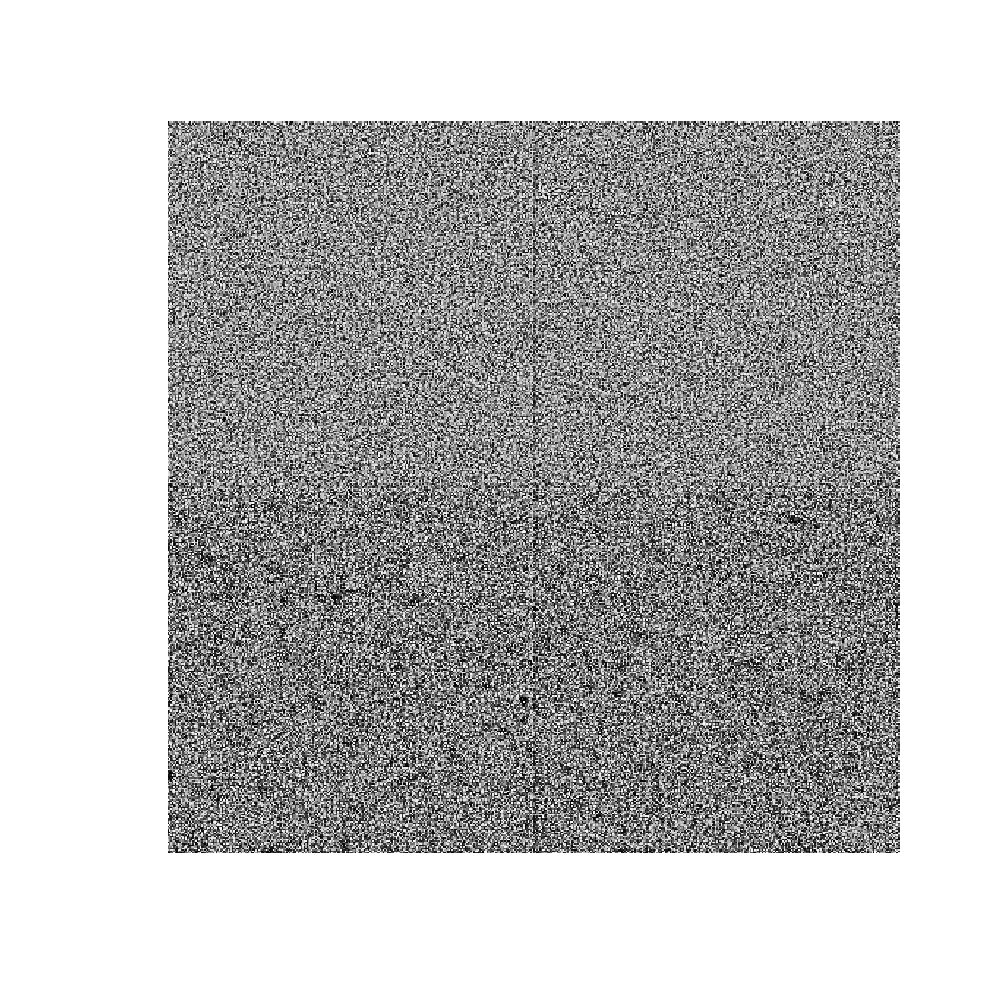
\includegraphics[scale=0.3]{../Figures/LEE/Cociente_CuatroZonas_EnhancedLee.pdf}}
	\caption{ENHANCED LEE}
\end{figure}






\begin{figure}[H]
	\centering
	\subfigure[\label{N1-h2-9x3}$N1-h2-9x3$]{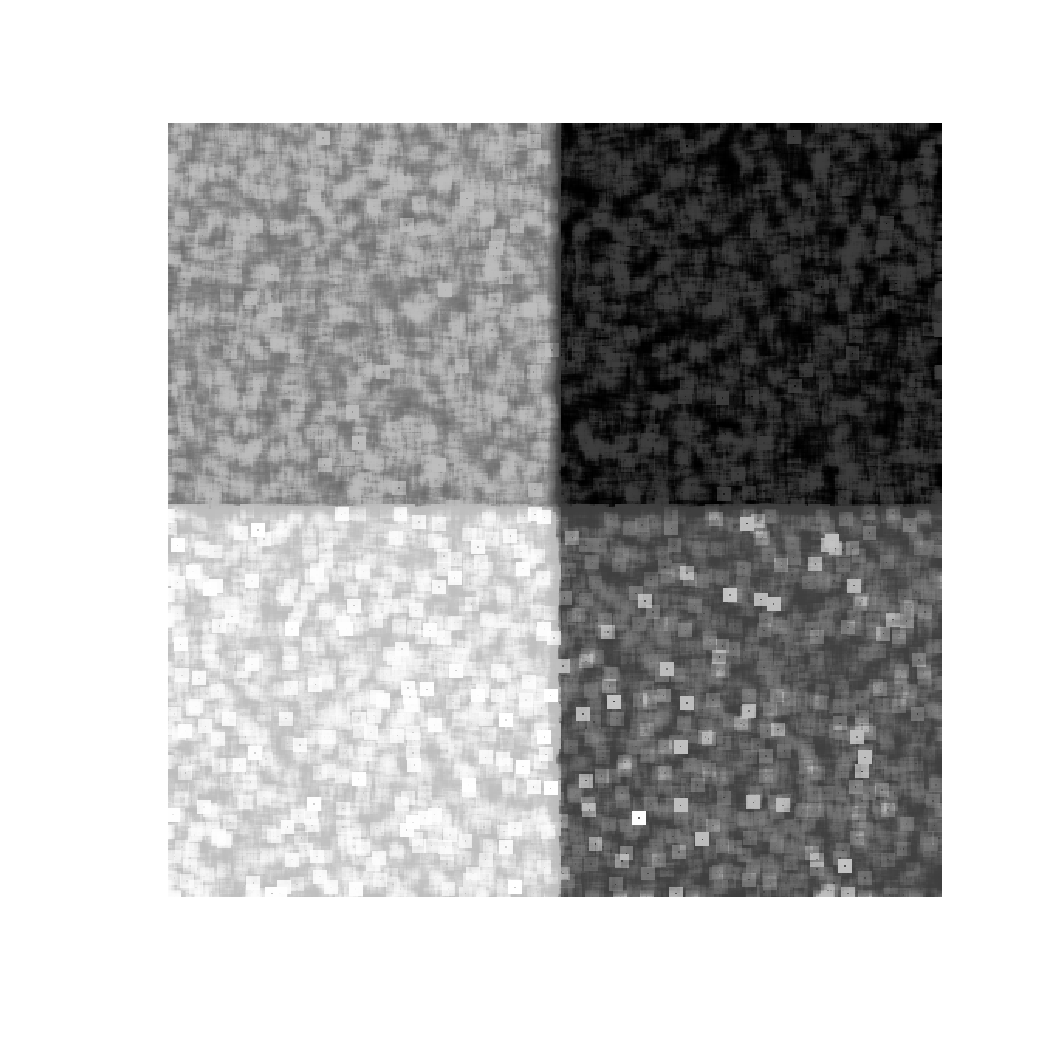
\includegraphics[scale=0.3]{../Figures/9por3/CuatroZonas_N1_h2_9por3.pdf}}
	\subfigure[\label{N1-h3-9x3}$N1-h3-9x3$]{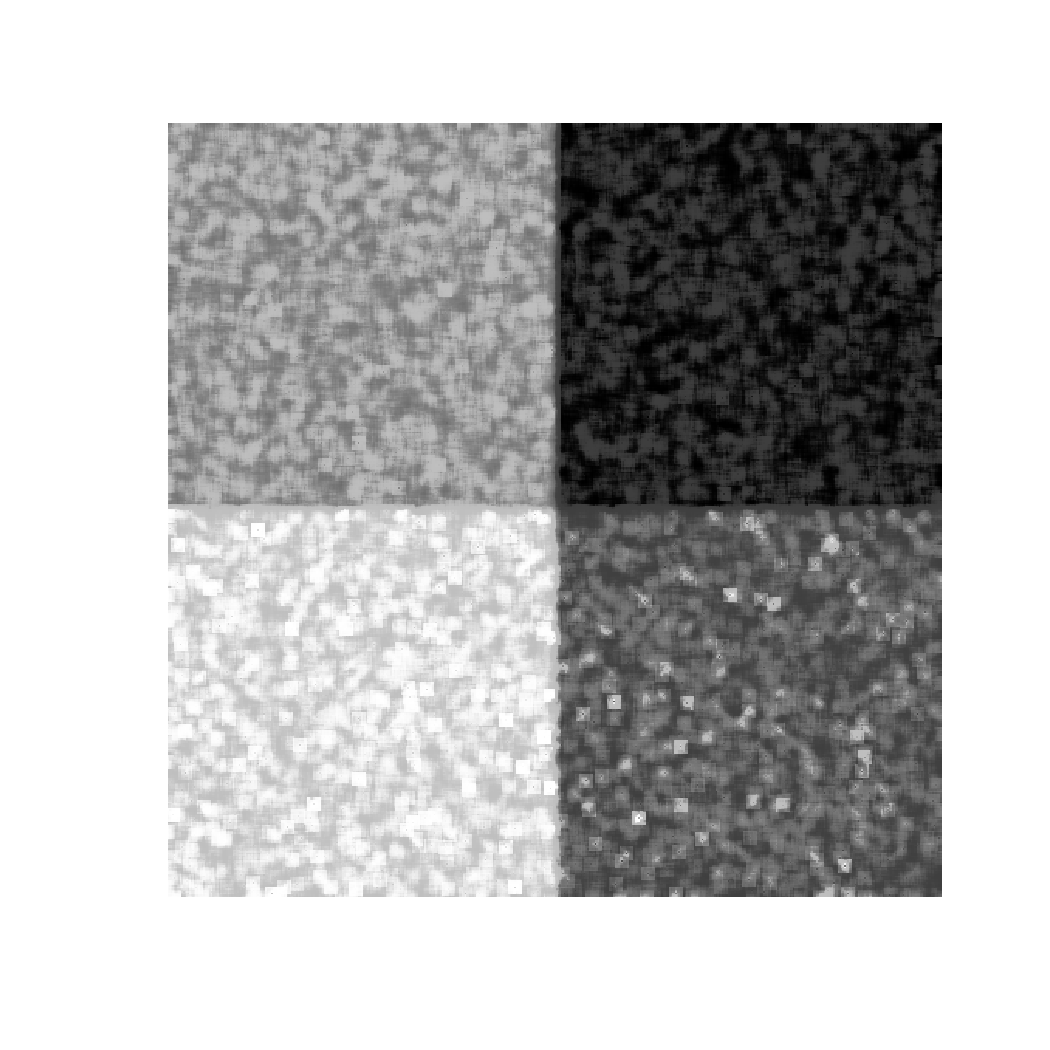
\includegraphics[scale=0.3]{../Figures/9por3/CuatroZonas_N1_h3_9por3.pdf}}
	\subfigure[\label{N1-h4-9x3}$N1-h4-9x3$]{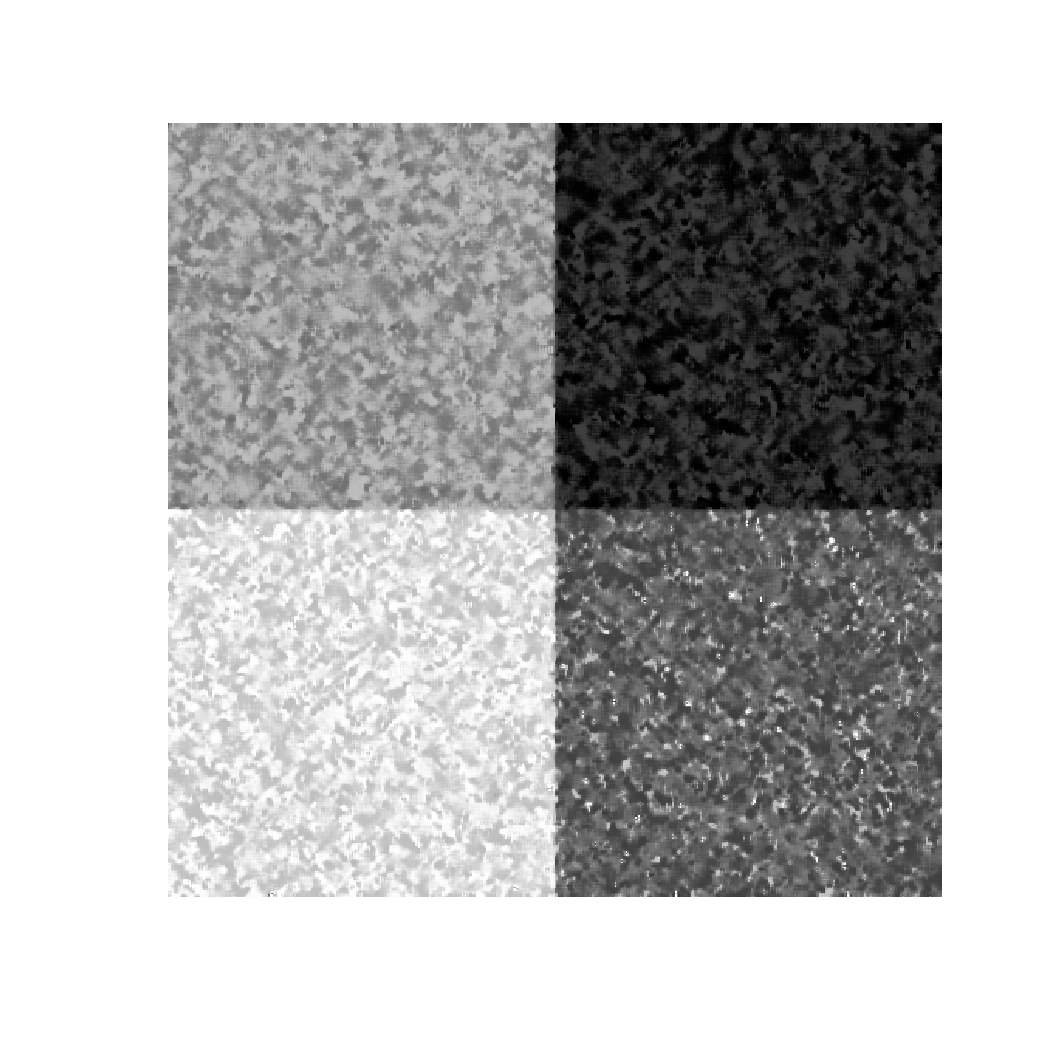
\includegraphics[scale=0.3]{../Figures/9por3/CuatroZonas_N1_h4_9por3.pdf}}
	\subfigure[\label{Cociente-N1-h2-9x3}Cociente-$N1-h2-9x3$]{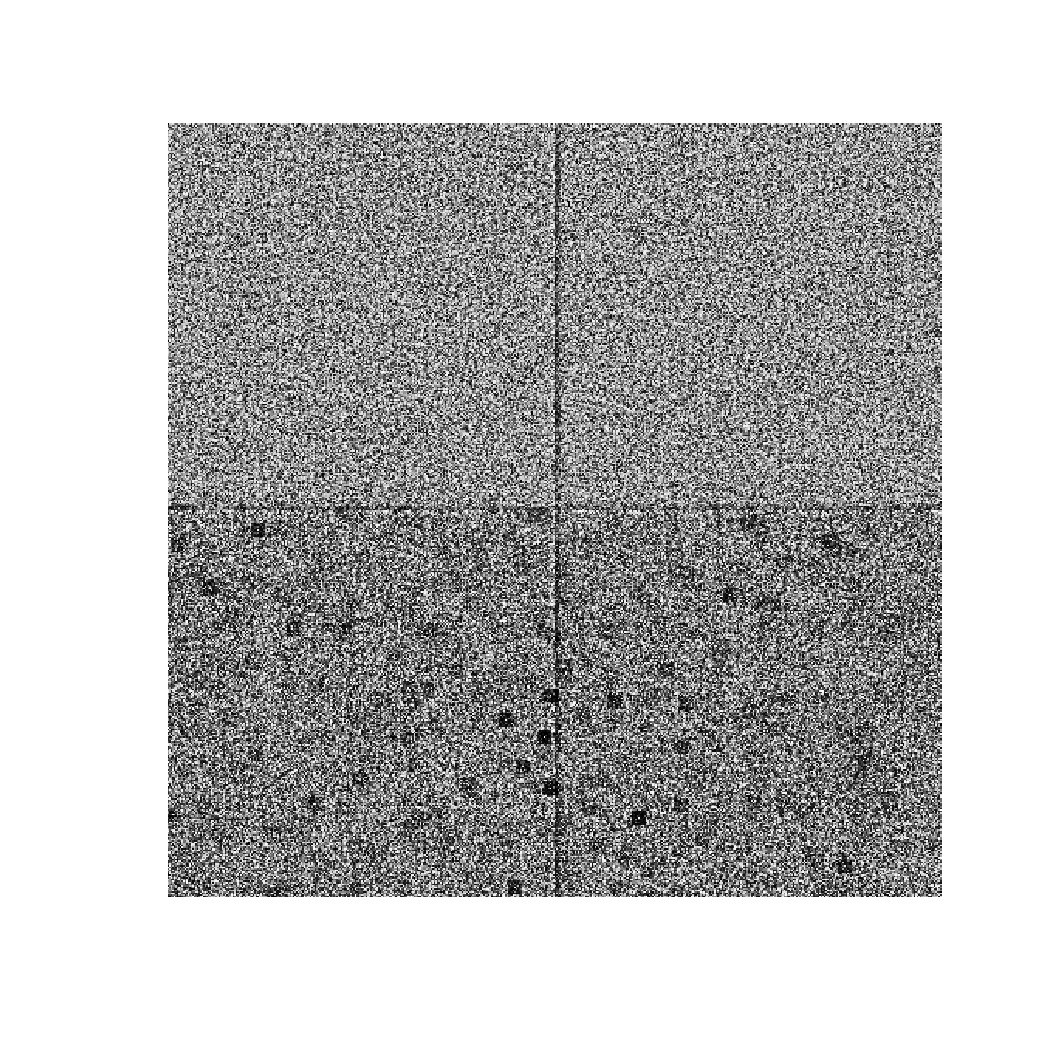
\includegraphics[scale=0.3]{../Figures/9por3/Cociente_CuatroZonas_N1_h2_9por3.pdf}}
	\subfigure[\label{Cociente-N1-h3-9x3}Cociente-$N1-h3-9x3$]{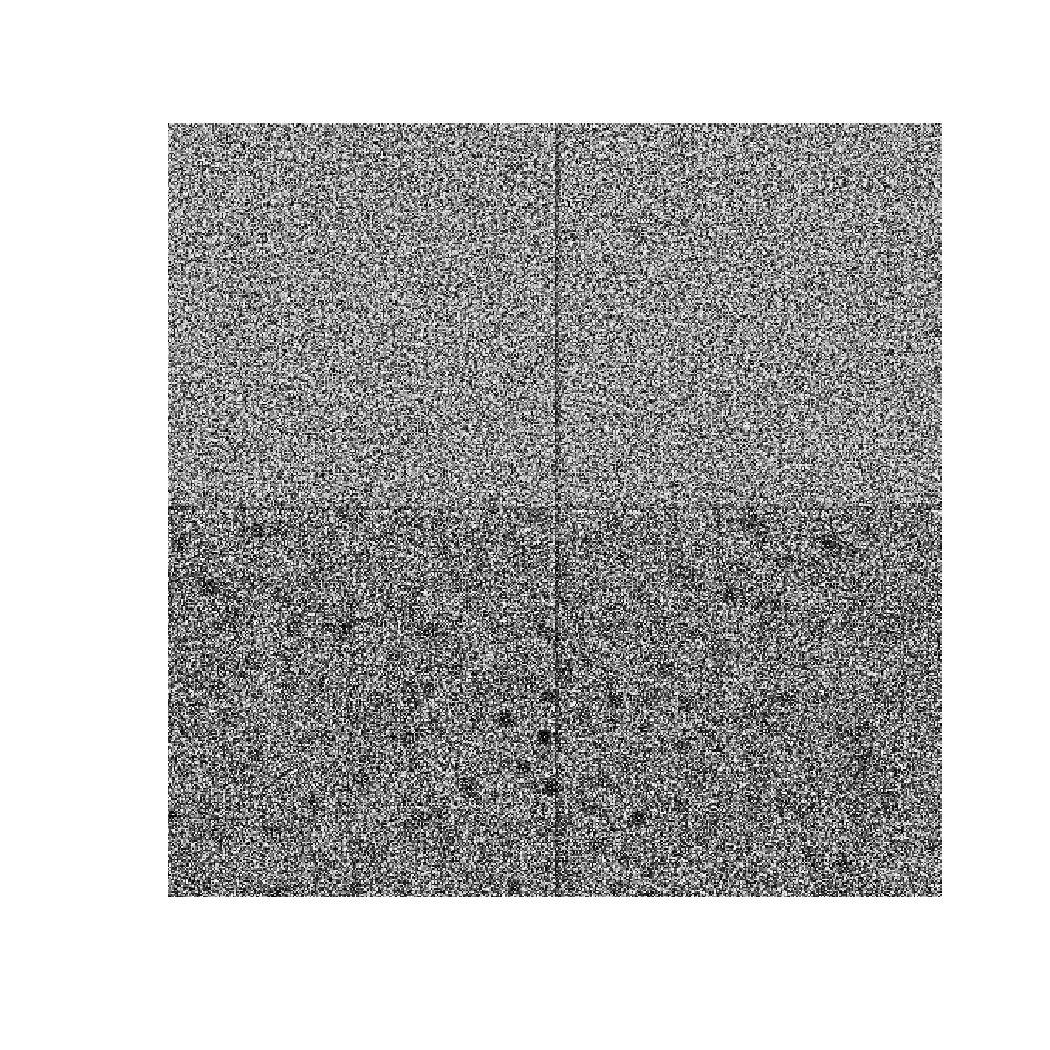
\includegraphics[scale=0.3]{../Figures/9por3/Cociente_CuatroZonas_N1_h3_9por3.pdf}}
	\subfigure[\label{Cociente-N1-h4-9x3}Cociente-$N1-h4-9x3$]{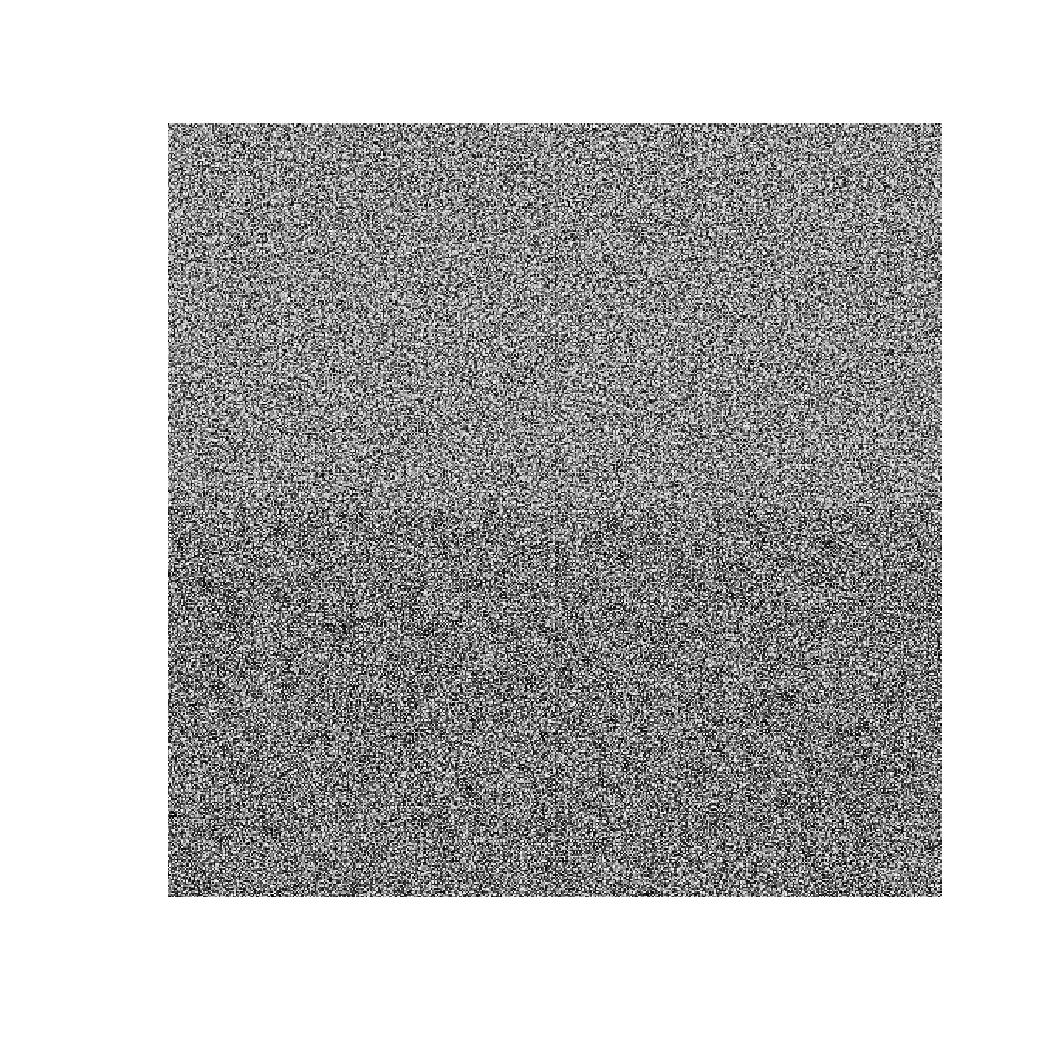
\includegraphics[scale=0.3]{../Figures/9por3/Cociente_CuatroZonas_N1_h4_9por3.pdf}}
	\caption{Our proposal 9x3}
\end{figure}  


\begin{figure}[H]
	\centering
	\subfigure[\label{N1-h2-9x5}$N1-h2-9x5$]{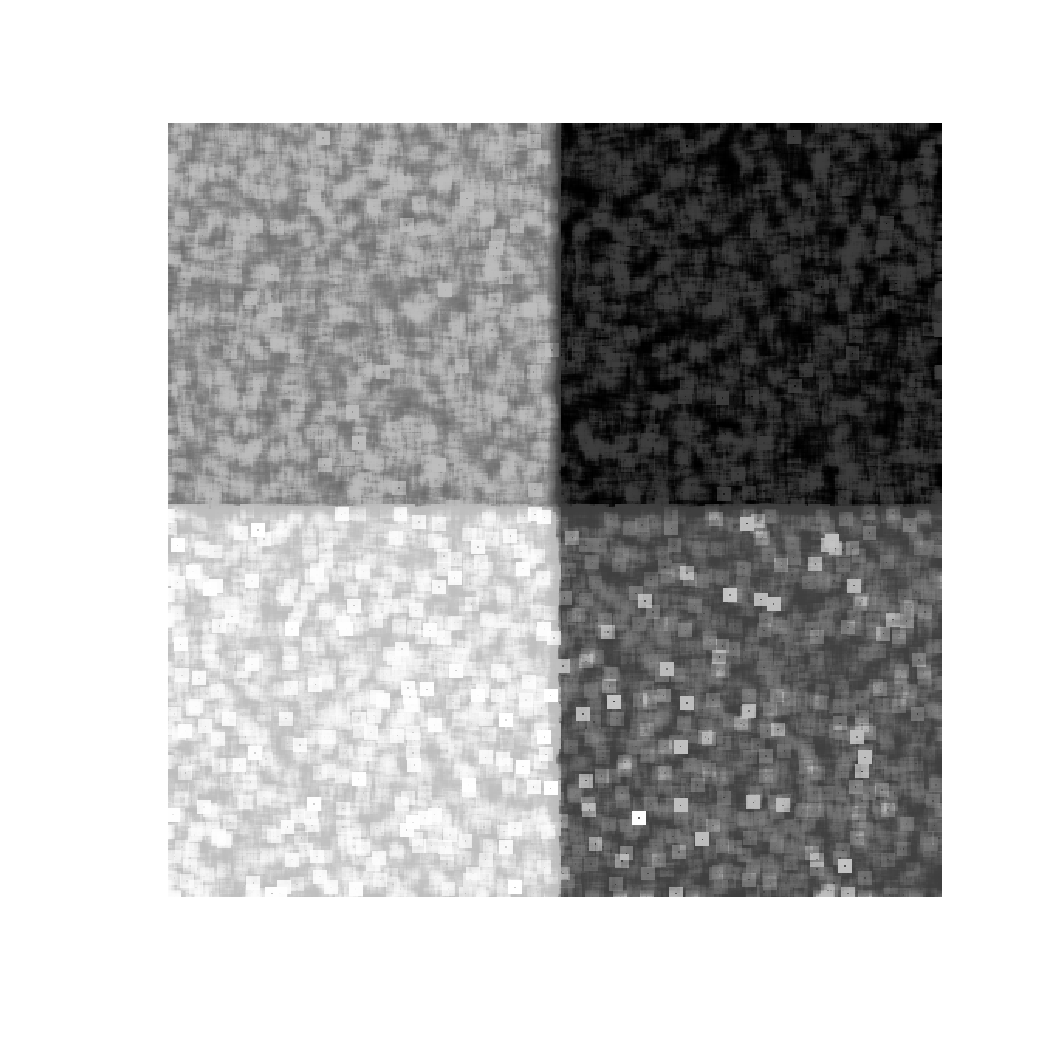
\includegraphics[scale=0.3]{../Figures/9por5/CuatroZonas_N1_h2_9por5.pdf}}
	\subfigure[\label{N1-h3-9x5}$N1-h3-9x5$]{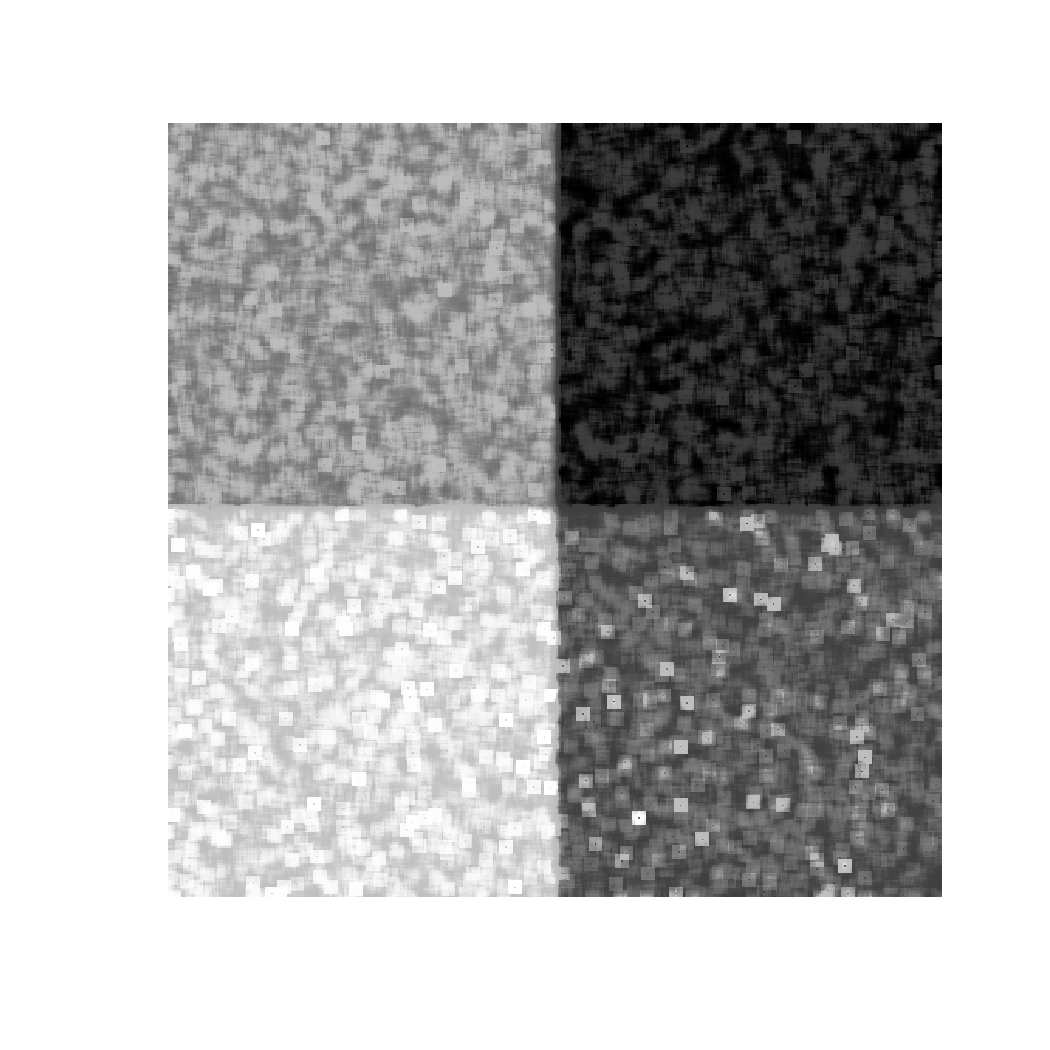
\includegraphics[scale=0.3]{../Figures/9por5/CuatroZonas_N1_h3_9por5.pdf}}
	\subfigure[\label{N1-h4-9x5}$N1-h4-9x5$]{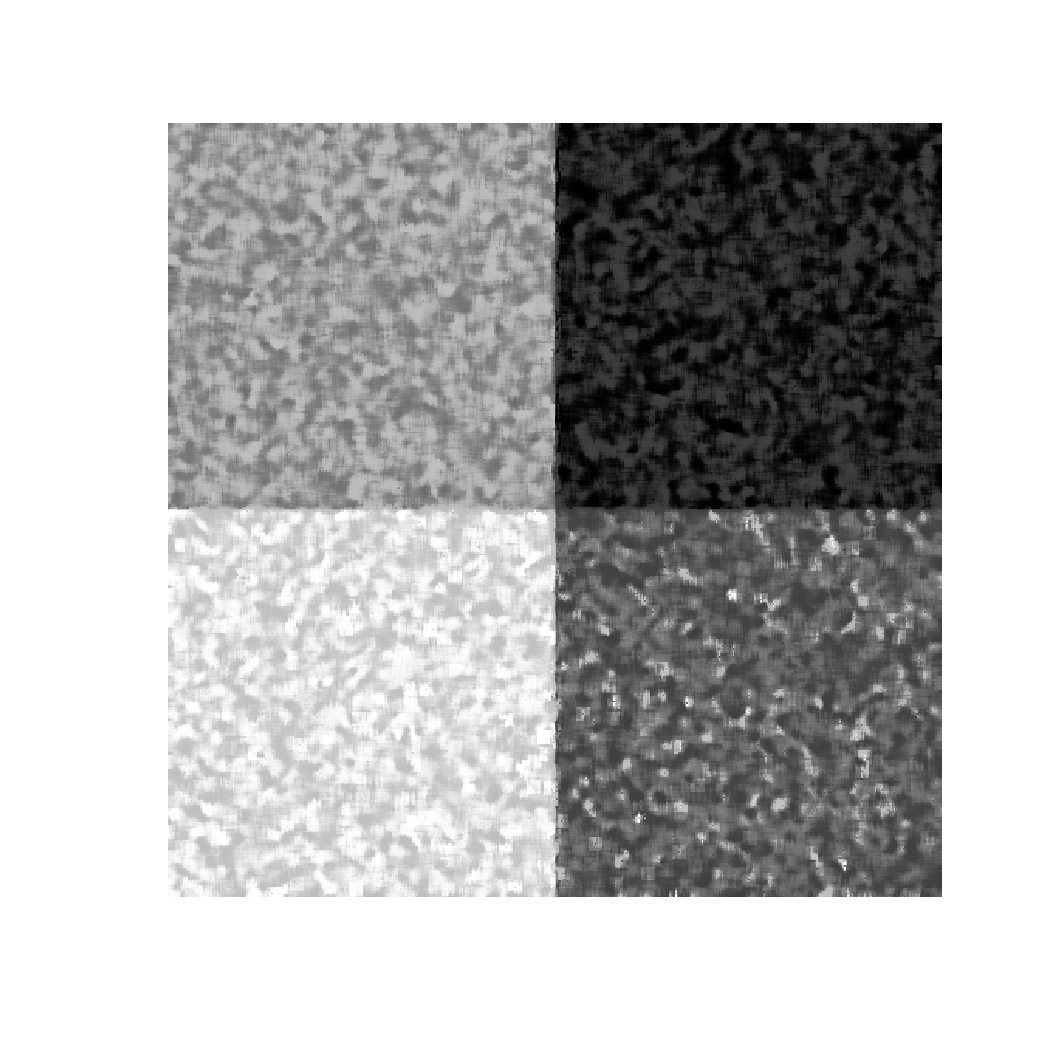
\includegraphics[scale=0.3]{../Figures/9por5/CuatroZonas_N1_h4_9por5.pdf}}
	\subfigure[\label{Cociente-N1-h2-9x5}Cociente-$N1-h2-9x5$]{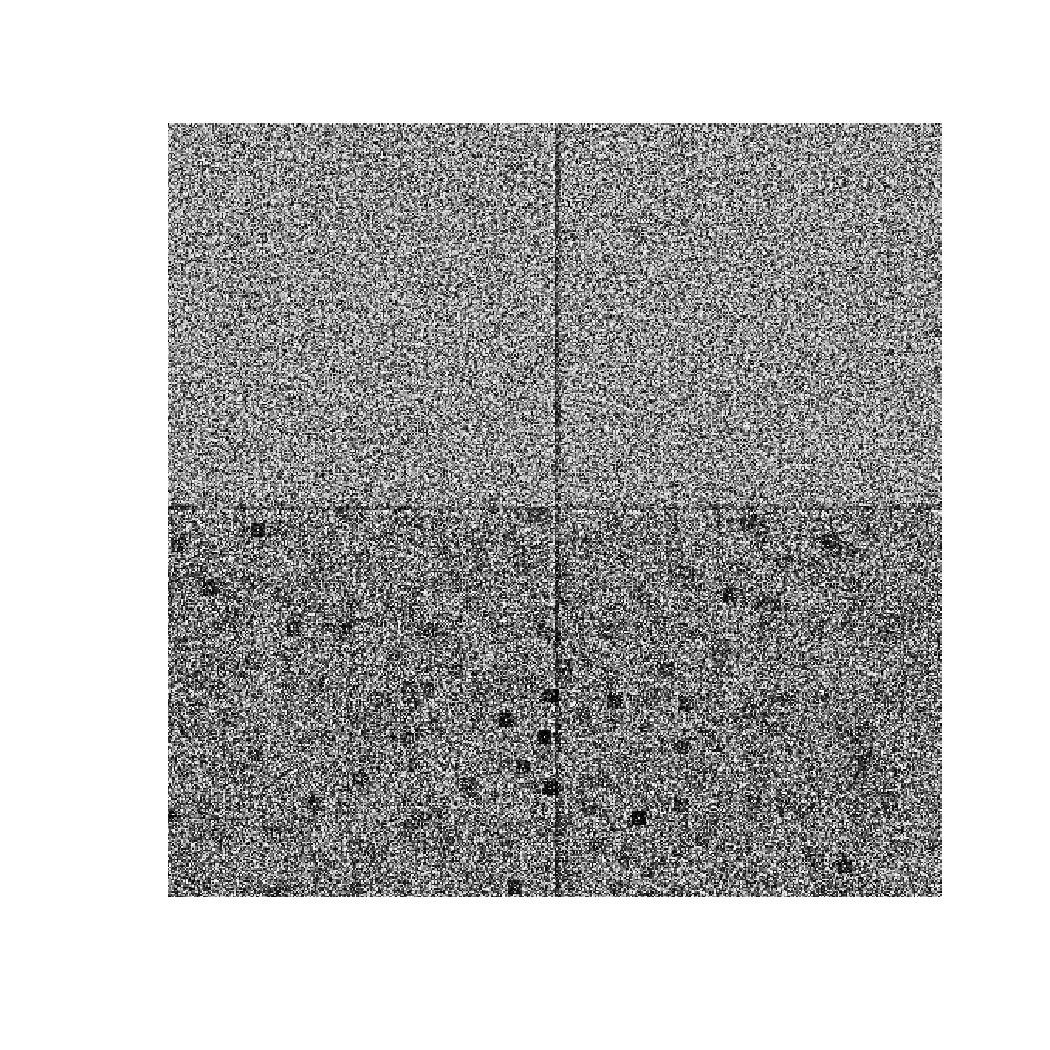
\includegraphics[scale=0.3]{../Figures/9por5/Cociente_CuatroZonas_N1_h2_9por5.pdf}}
	\subfigure[\label{Cociente-N1-h3-9x5}Cociente-$N1-h3-9x5$]{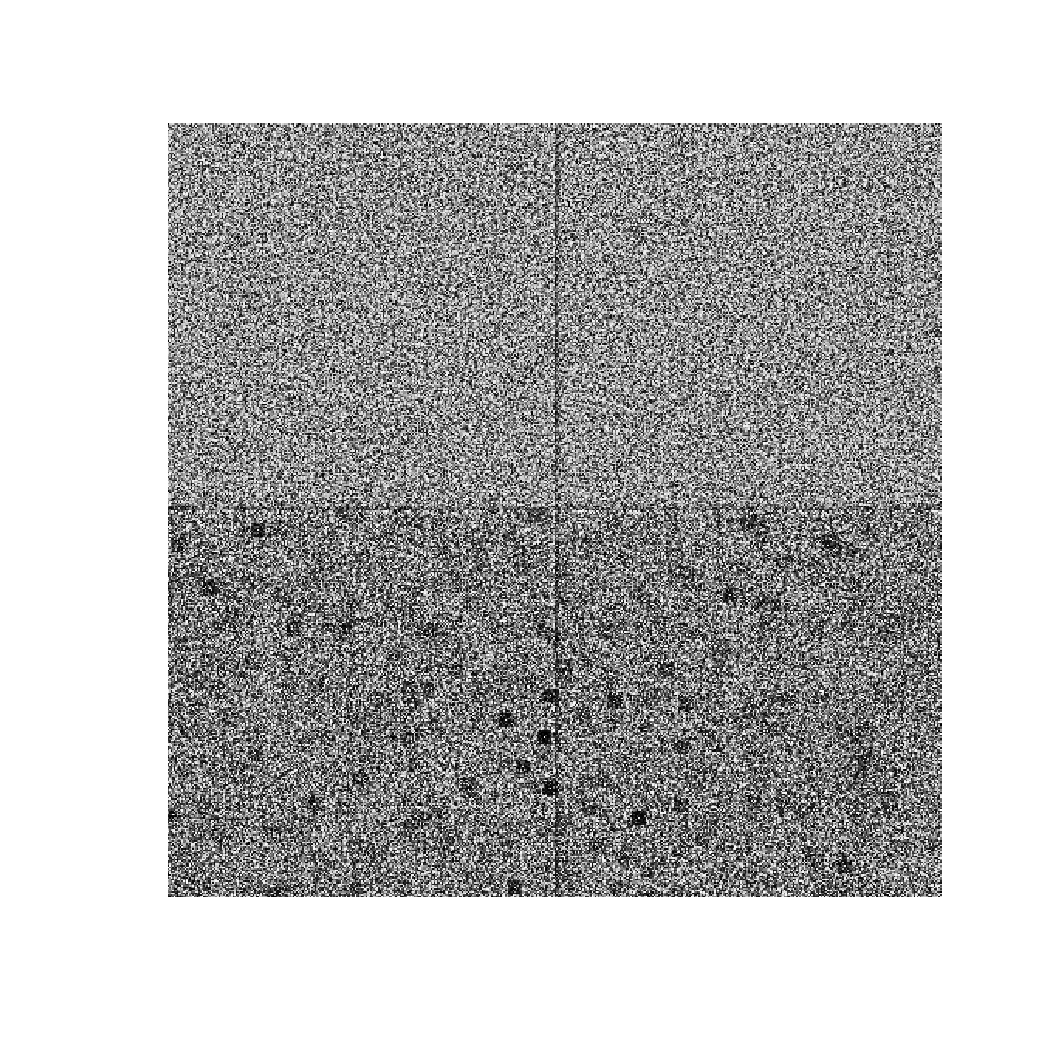
\includegraphics[scale=0.3]{../Figures/9por5/Cociente_CuatroZonas_N1_h3_9por5.pdf}}
	\subfigure[\label{Cociente-N1-h4-9x5}Cociente-$N1-h4-9x5$]{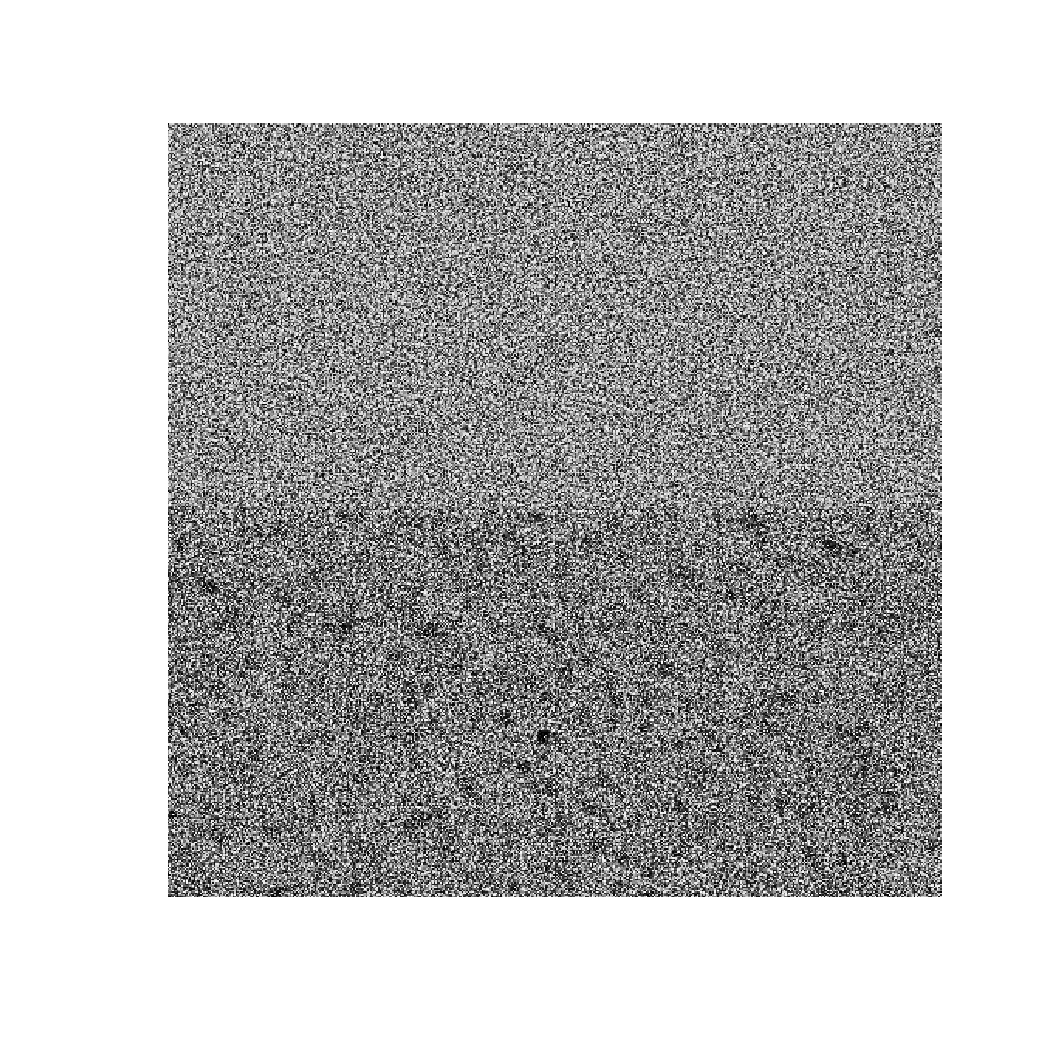
\includegraphics[scale=0.3]{../Figures/9por5/Cociente_CuatroZonas_N1_h4_9por5.pdf}}
	\caption{Our proposal 9x5}
\end{figure}  


\begin{figure}[H]
	\centering
	\subfigure[\label{N1-h2-11x7}$N1-h2-11x7$]{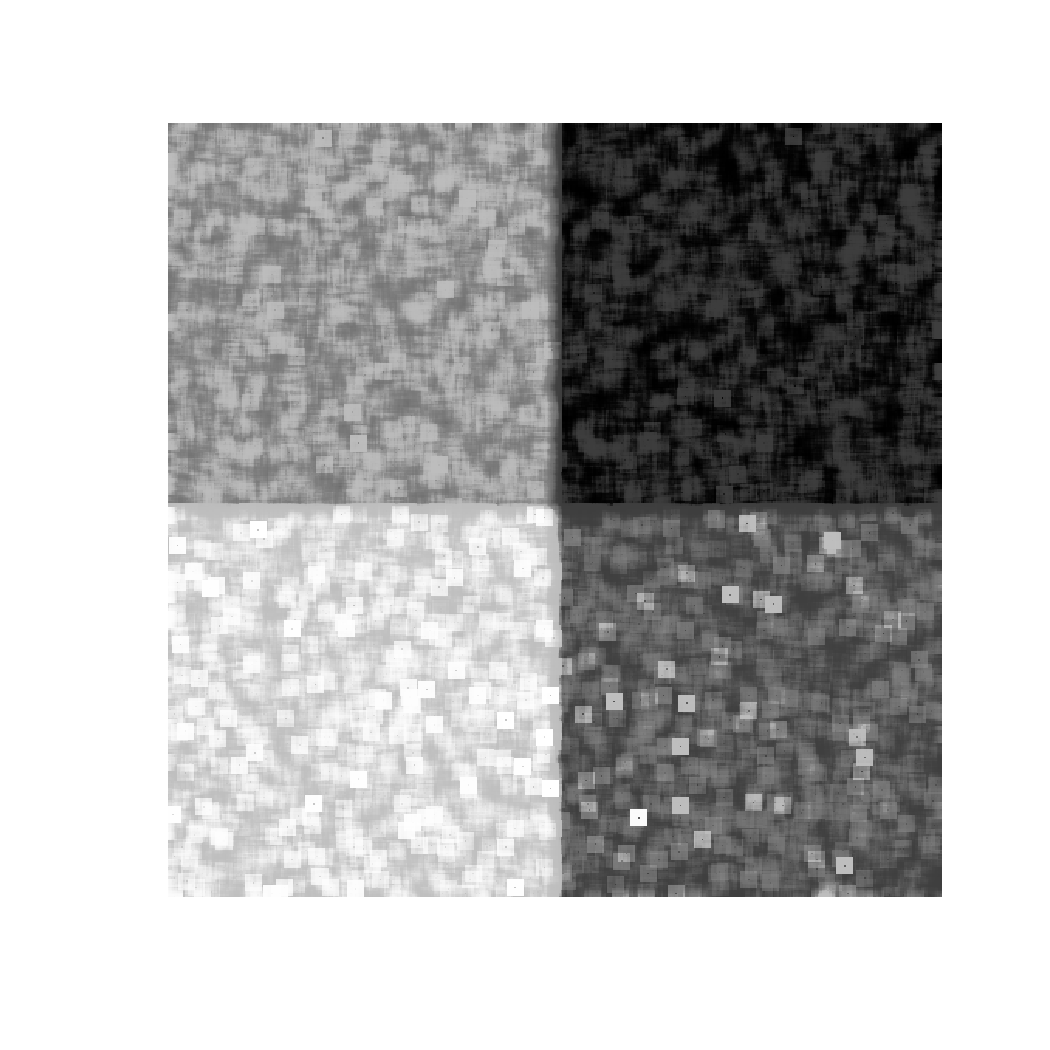
\includegraphics[scale=0.3]{../Figures/11por7/CuatroZonas_N1_h2_11por7.pdf}}
	\subfigure[\label{N1-h3-11x7}$N1-h3-11x7$]{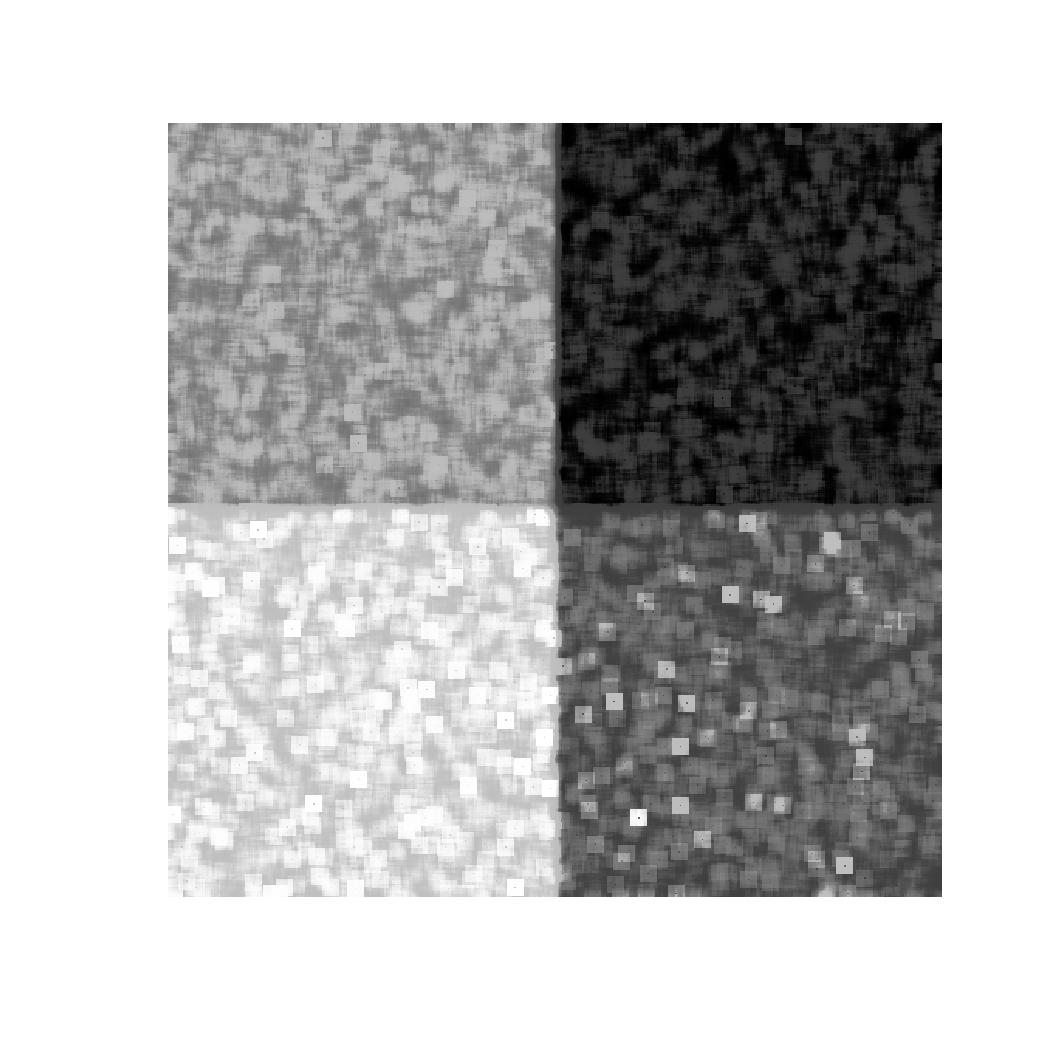
\includegraphics[scale=0.3]{../Figures/11por7/CuatroZonas_N1_h3_11por7.pdf}}
	\subfigure[\label{N1-h4-11x7}$N1-h4-11x7$]{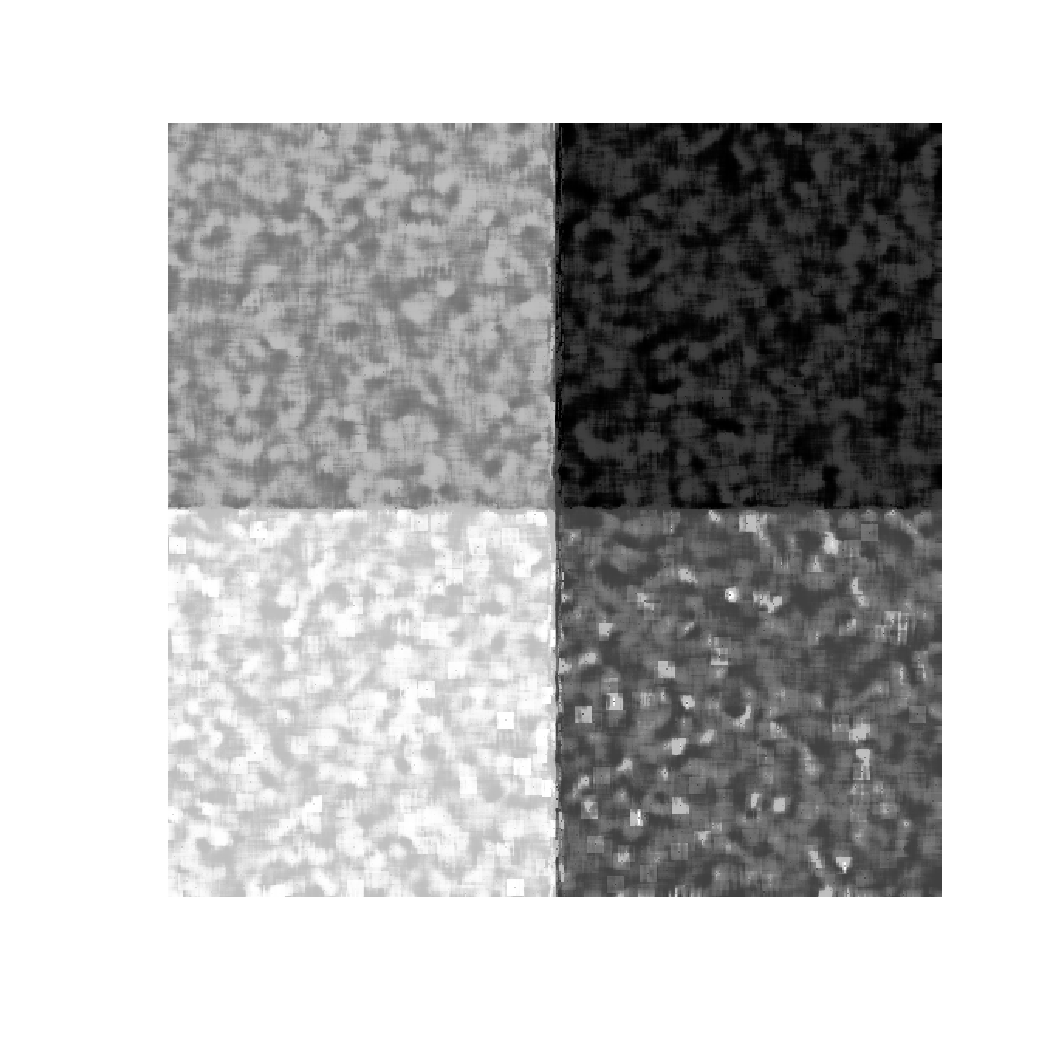
\includegraphics[scale=0.3]{../Figures/11por7/CuatroZonas_N1_h4_11por7.pdf}}
	\subfigure[\label{Cociente-N1-h2-11x7}Cociente-$N1-h2-11x7$]{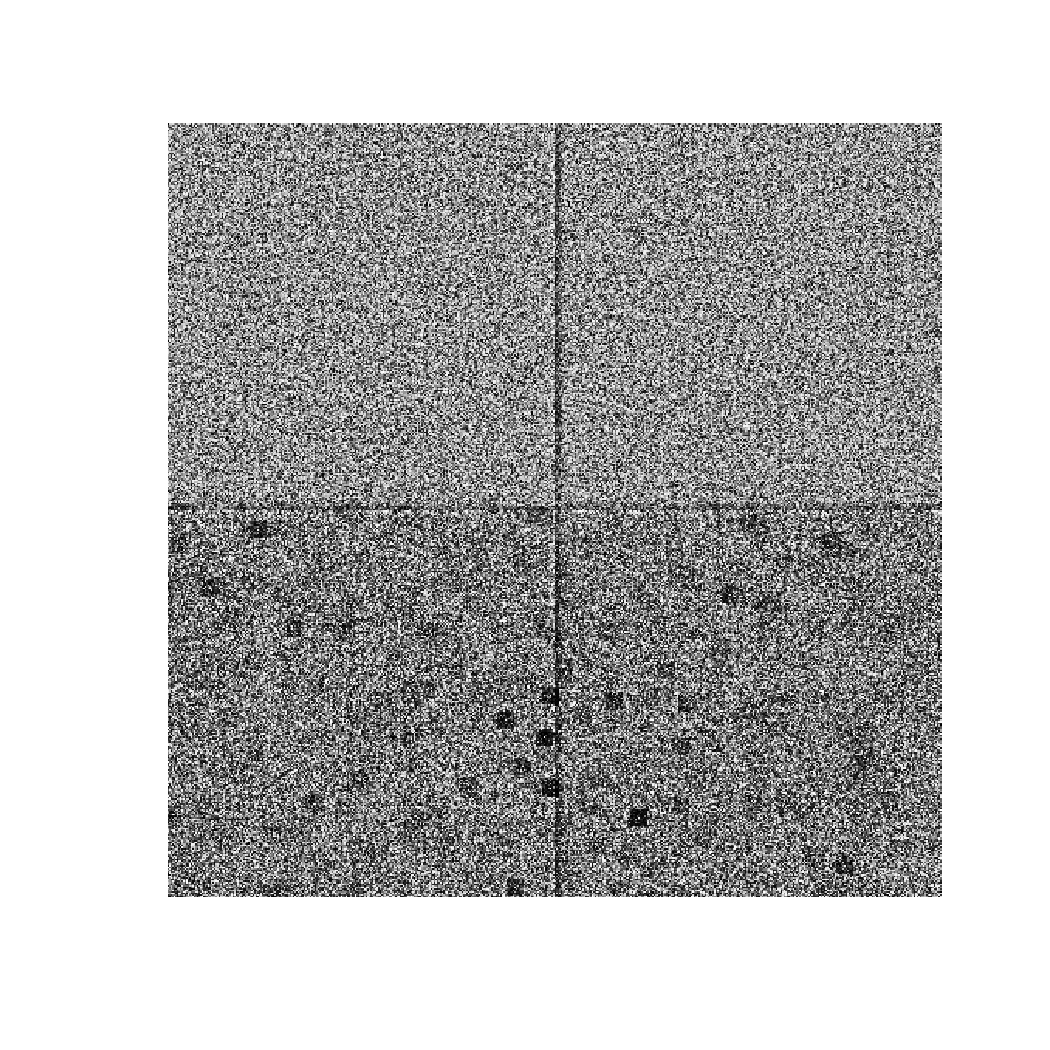
\includegraphics[scale=0.3]{../Figures/11por7/Cociente_CuatroZonas_N1_h2_11por7.pdf}}
	\subfigure[\label{Cociente-N1-h3-11x7}Cociente-$N1-h3-11x7$]{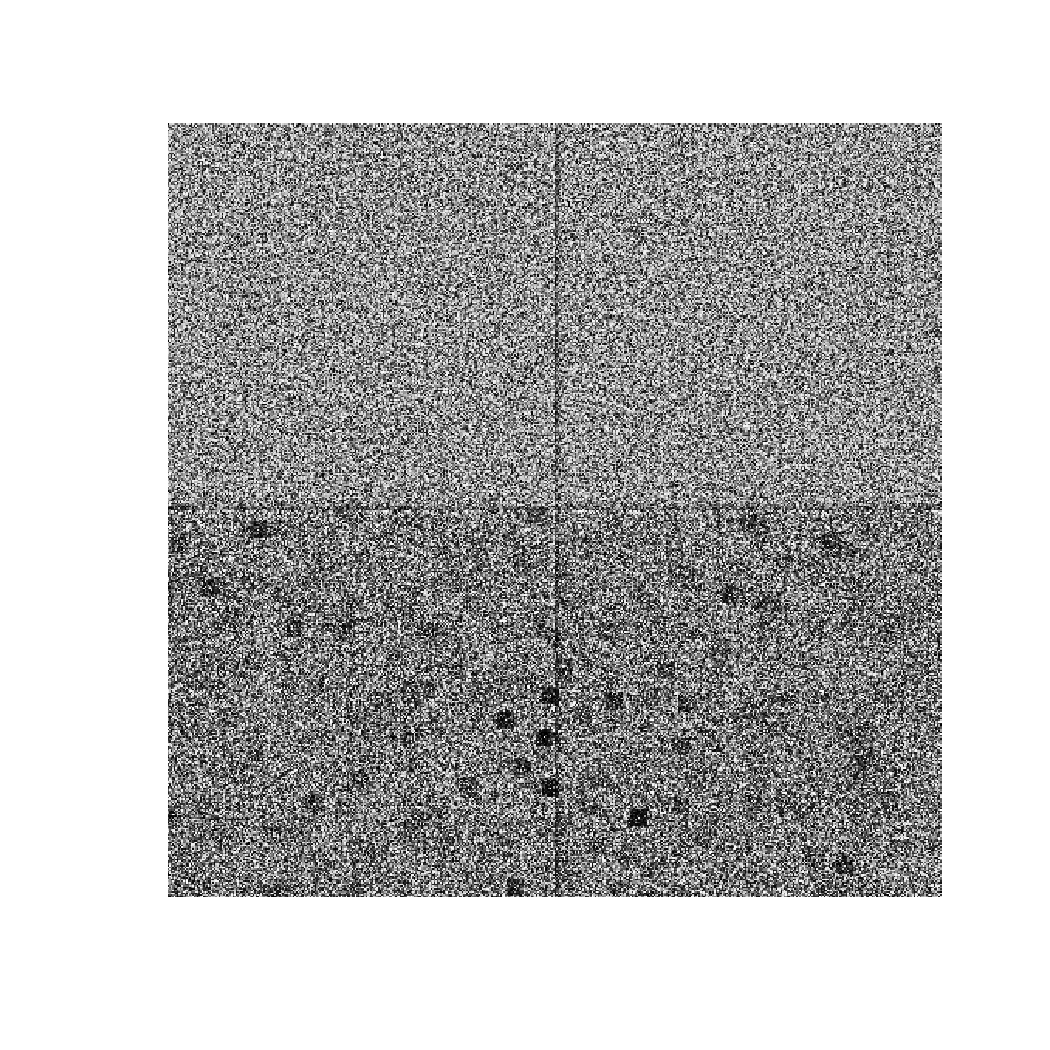
\includegraphics[scale=0.3]{../Figures/11por7/Cociente_CuatroZonas_N1_h3_11por7.pdf}}
	\subfigure[\label{Cociente-N1-h4-11x7}Cociente-$N1-h4-11x7$]{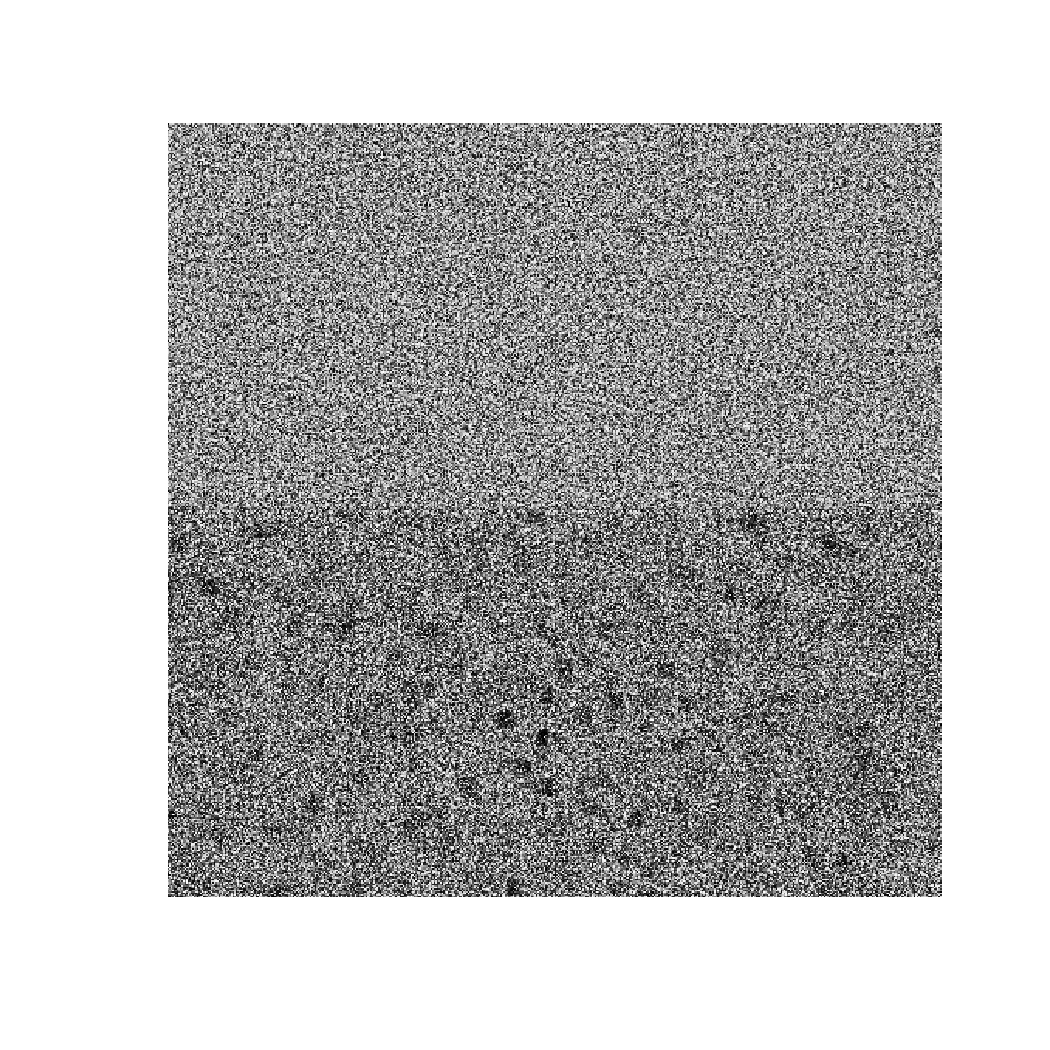
\includegraphics[scale=0.3]{../Figures/11por7/Cociente_CuatroZonas_N1_h4_11por7.pdf}}
	\caption{Our proposal 11x7}
\end{figure}  
\end{document}

